\newpage
\hypertarget{conBran tex}{}
\subsection{Branching via}
\texHeader

\begin{itemize}

\item[$\blacktriangleright$] Before doing anything else, lets declare the method that will insert two new partitions into \texttt{box} when the original pattern
match fails. Open \texttt{Box.eclass} and write the following signature: 
\syntax{initializeBox () : EBoolean}

\vspace{0.5cm}

\item[$\blacktriangleright$] Now we need to modify \texttt{Box.grow()} with nested \emph{if/else} constructs, where \texttt{[addNewPartitionBox]} is the first
conditional, and a statement node is the second. Your EClass should now include Fig.~\ref{fig:updateGrow}

\vspace{0.5cm}

\begin{figure}[htp]
\begin{center}
  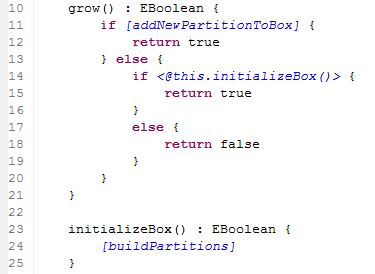
\includegraphics[width=0.5\textwidth]{eclipse_updateGrow}
  \caption{Extending \texttt{box.grow()}}
  \label{fig:updateGrow}
\end{center}
\end{figure}

\vspace{0.5cm}

\item[$\blacktriangleright$] Easy! Now, we want to define our newest method. As we mentioned before, you now have a choice -- you can either write the Java
implementation yourself in \texttt{Box.impl}, or continue as we have construct a pattern. Given that this uses an NAC, let's do it the way we already know by
creating a \texttt{[buildPartitions]} pattern.

\vspace{0.5cm}

\item[$\blacktriangleright$] Open and complete \texttt{[buildPartitions]} as illustrated in Fig.~\ref{fig:pattBuildParts}. As you can see, we have a bounded
box to check and see if a connection to \texttt{onePartition} exists. If none exists, the pattern will proceed to create a \texttt{firstPartition} and
\texttt{lastPartition}, and set up their references accordingly.

\clearpage

\vspace*{2cm}

\begin{figure}[htp]
\begin{center}
  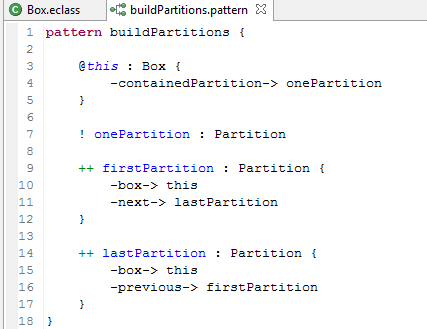
\includegraphics[width=0.7\textwidth]{eclipse_buildPartitionsPattern}
  \caption{Pattern to check for only \texttt{one} partition.}
  \label{fig:pattBuildParts}
\end{center}
\end{figure}

\item[$\blacktriangleright$] That's everything! Save and build your metamodel to make sure no errors exist.

\end{itemize}
